\documentclass{ximera}
\usepackage{longdivision}
\usepackage{polynom}
\usepackage{float}% Use `H' as the figure optional argument to force it's vertical placement to conform to source.
%\usepackage{caption}% Allows us to describe the figures without having "figure 1:" in it. :: Apparently Caption isn't supported.
%    \captionsetup{labelformat=empty}% Actually does the figure configuration stated above.
\usetikzlibrary{arrows.meta,arrows}% Allow nicer arrow heads for tikz.
\usepackage{gensymb, pgfplots}
\usepackage{tabularx}
\usepackage{arydshln}
\usepackage[margin=1.5cm]{geometry}
\usepackage{indentfirst}

\setlength\parindent{16pt}

\graphicspath{
  {./}
  {./explorePolynomials/}
  {./exploreRadicals/}
  {./graphing/}
}

%% Default style for tikZ
\pgfplotsset{my style/.append style={axis x line=middle, axis y line=
middle, xlabel={$x$}, ylabel={$y$}, axis equal }}


%% Because log being natural log is too hard for people.
\let\logOld\log% Keep the old \log definition, just in case we need it.
\renewcommand{\log}{\ln}


%%% Changes in polynom to show the zero coefficient terms
\makeatletter
\def\pld@CF@loop#1+{%
    \ifx\relax#1\else
        \begingroup
          \pld@AccuSetX11%
          \def\pld@frac{{}{}}\let\pld@symbols\@empty\let\pld@vars\@empty
          \pld@false
          #1%
          \let\pld@temp\@empty
          \pld@AccuIfOne{}{\pld@AccuGet\pld@temp
                            \edef\pld@temp{\noexpand\pld@R\pld@temp}}%
           \pld@if \pld@Extend\pld@temp{\expandafter\pld@F\pld@frac}\fi
           \expandafter\pld@CF@loop@\pld@symbols\relax\@empty
           \expandafter\pld@CF@loop@\pld@vars\relax\@empty
           \ifx\@empty\pld@temp
               \def\pld@temp{\pld@R11}%
           \fi
          \global\let\@gtempa\pld@temp
        \endgroup
        \ifx\@empty\@gtempa\else
            \pld@ExtendPoly\pld@tempoly\@gtempa
        \fi
        \expandafter\pld@CF@loop
    \fi}
\def\pld@CMAddToTempoly{%
    \pld@AccuGet\pld@temp\edef\pld@temp{\noexpand\pld@R\pld@temp}%
    \pld@CondenseMonomials\pld@false\pld@symbols
    \ifx\pld@symbols\@empty \else
        \pld@ExtendPoly\pld@temp\pld@symbols
    \fi
    \ifx\pld@temp\@empty \else
        \pld@if
            \expandafter\pld@IfSum\expandafter{\pld@temp}%
                {\expandafter\def\expandafter\pld@temp\expandafter
                    {\expandafter\pld@F\expandafter{\pld@temp}{}}}%
                {}%
        \fi
        \pld@ExtendPoly\pld@tempoly\pld@temp
        \pld@Extend\pld@tempoly{\pld@monom}%
    \fi}
\makeatother




%%%%% Code for making prime factor trees for numbers, taken from user Qrrbrbirlbel at: https://tex.stackexchange.com/questions/131689/how-to-automatically-draw-tree-diagram-of-prime-factorization-with-latex

\usepackage{forest,mathtools,siunitx}
\makeatletter
\def\ifNum#1{\ifnum#1\relax
  \expandafter\pgfutil@firstoftwo\else
  \expandafter\pgfutil@secondoftwo\fi}
\forestset{
  num content/.style={
    delay={
      content/.expanded={\noexpand\num{\forestoption{content}}}}},
  pt@prime/.style={draw, circle},
  pt@start/.style={},
  pt@normal/.style={},
  start primeTree/.style={%
    /utils/exec=%
      % \pt@start holds the current minimum factor, we'll start with 2
      \def\pt@start{2}%
      % \pt@result will hold the to-be-typeset factorization, we'll start with
      % \pgfutil@gobble since we don't want a initial \times
      \let\pt@result\pgfutil@gobble
      % \pt@start@cnt holds the number of ^factors for the current factor
      \def\pt@start@cnt{0}%
      % \pt@lStart will later hold "l"ast factor used
      \let\pt@lStart\pgfutil@empty,
    alias=pt-start,
    pt@start/.try,
    delay={content/.expanded={$\noexpand\num{\forestove{content}}
                            \noexpand\mathrlap{{}= \noexpand\pt@result}$}},
    primeTree},
  primeTree/.code=%
    % take the content of the node and save it in the count
    \c@pgf@counta\forestove{content}\relax
    % if it's 2 we're already finished with the factorization
    \ifNum{\c@pgf@counta=2}{%
      % add the factor
      \pt@addfactor{2}%
      % finalize the factorization of the result
      \pt@addfactor{}%
      % and set the style to the prime style
      \forestset{pt@prime/.try}%
    }{%
      % this simply calculates content/2 and saves it in \pt@end
      % this is later used for an early break of the recursion since no factor
      % can be greater then content/2 (for integers of course)
      \edef\pt@content{\the\c@pgf@counta}%
      \divide\c@pgf@counta2\relax
      \advance\c@pgf@counta1\relax % to be on the safe side
      \edef\pt@end{\the\c@pgf@counta}%
      \pt@do}}

%%% our main "function"
\def\pt@do{%
  % let's test if the current factor is already greather then the max factor
  \ifNum{\pt@end<\pt@start}{%
    % great, we're finished, the same as above
    \expandafter\pt@addfactor\expandafter{\pt@content}%
    \pt@addfactor{}%
    \def\pt@next{\forestset{pt@prime/.try}}%
  }{%
    % this calculates int(content/factor)*factor
    % if factor is a factor of content (without remainder), the result will
    % equal content. The int(content/factor) is saved in \pgf@temp.
    \c@pgf@counta\pt@content\relax
    \divide\c@pgf@counta\pt@start\relax
    \edef\pgf@temp{\the\c@pgf@counta}%
    \multiply\c@pgf@counta\pt@start\relax
    \ifNum{\the\c@pgf@counta=\pt@content}{%
      % yeah, we found a factor, add it to the result and ...
      \expandafter\pt@addfactor\expandafter{\pt@start}%
      % ... add the factor as the first child with style pt@prime
      % and the result of int(content/factor) as another child.
      \edef\pt@next{\noexpand\forestset{%
        append={[\pt@start, pt@prime/.try]},
        append={[\pgf@temp, pt@normal/.try]},
        % forest is complex, this makes sure that for the second child, the
        % primeTree style is not executed too early (there must be a better way).
        delay={
          for descendants={
            delay={if n'=1{primeTree, num content}{}}}}}}%
    }{%
      % Alright this is not a factor, let's get the next factor
      \ifNum{\pt@start=2}{%
        % if the previous factor was 2, the next one will be 3
        \def\pt@start{3}%
      }{%
        % hmm, the previos factor was not 2,
        % let's add 2, maybe we'll hit the next prime number
        % and maybe a factor
        \c@pgf@counta\pt@start
        \advance\c@pgf@counta2\relax
        \edef\pt@start{\the\c@pgf@counta}%
      }%
      % let's do that again
      \let\pt@next\pt@do
    }%
  }%
  \pt@next
}

%%% this builds the \pt@result macro with the factors
\def\pt@addfactor#1{%
  \def\pgf@tempa{#1}%
  % is it the same factor as the previous one
  \ifx\pgf@tempa\pt@lStart
    % add 1 to the counter
    \c@pgf@counta\pt@start@cnt\relax
    \advance\c@pgf@counta1\relax
    \edef\pt@start@cnt{\the\c@pgf@counta}%
  \else
    % a new factor! Add the previous one to the product of factors
    \ifx\pt@lStart\pgfutil@empty\else
      % as long as there actually is one, the \ifnum makes sure we do not add ^1
      \edef\pgf@tempa{\noexpand\num{\pt@lStart}\ifnum\pt@start@cnt>1 
                                           ^{\noexpand\num{\pt@start@cnt}}\fi}%
      \expandafter\pt@addfactor@\expandafter{\pgf@tempa}%
    \fi
    % setup the macros for the next round
    \def\pt@lStart{#1}% <- current (new) factor
    \def\pt@start@cnt{1}% <- first time
  \fi
}
%%% This simply appends "\times #1" to \pt@result, with etoolbox this would be
%%% \appto\pt@result{\times#1}
\def\pt@addfactor@#1{%
  \expandafter\def\expandafter\pt@result\expandafter{\pt@result \times #1}}

%%% Our main macro:
%%% #1 = possible optional argument for forest (can be tikz too)
%%% #2 = the number to factorize
\newcommand*{\PrimeTree}[2][]{%
  \begin{forest}%
    % as the result is set via \mathrlap it doesn't update the bounding box
    % let's fix this:
    tikz={execute at end scope={\pgfmathparse{width("${}=\pt@result$")}%
                         \path ([xshift=\pgfmathresult pt]pt-start.east);}},
    % other optional arguments
    #1
    % And go!
    [#2, start primeTree]
  \end{forest}}
\makeatother


\providecommand\tabitem{\makebox[1em][r]{\textbullet~}}
\providecommand{\letterPlus}{\makebox[0pt][l]{$+$}}
\providecommand{\letterMinus}{\makebox[0pt][l]{$-$}}

\renewcommand{\texttt}[1]{#1}% Renew the command to prevent it from showing up in the sage strings for some weird reason.
%\renewcommand{\text}[1]{#1}% Renew the command to prevent it from showing up in the sage strings for some weird reason.



\title{Inverse Functions}
\begin{document}
\begin{abstract}
    This section introduces the geometric viewpoint of invertability.
\end{abstract}
\maketitle

\subsection*{Inverse Functions - Geometric View}

A recurring perspective as we move toward studying individual functions types will be the idea of \textit{inverting} a function. Remember that a function is a relationship between some domain and a codomain, where it ``maps" each domain point to a (single) point in the codomain. 

\begin{center}
    \begin{tikzpicture}[scale=2,filled dot/.style = {anchor=base,fill,circle,inner sep=0.5pt}]
        \draw plot [smooth cycle] coordinates {(0,0) (1,0.1) (2,0.3) (2,1.4) (1.5,2.5) (0.8,2.5) (0.3,1.2) (-0.2,0.6) } node at (1,1) {Domain};
        \draw plot [smooth cycle] coordinates {(4,0) (5,0.1) (6,0.3) (6,1.4) (5.5,2.5) (4.8,2.5) (4.3,1.2) (3.8,0.6) } node at (5,1) {Codomain};
        \draw[-{Latex[length=3mm]}] plot [smooth,tension=1.2] coordinates {(1,1.5) (3,2.5) (5,1.5)} node at (3,2.7) {$f(x)$} node [filled dot] at (1,1.5){.}  node at (1,1.35) {$x_1$} node at (5,1.4) {$y_1$};
    \end{tikzpicture}
\end{center}

Inverting a function is ``merely"%
\footnote{%
    Like most things, ``merely" is entirely misleading here... in fact this tends to be the hard part, and doesn't always work, as we'll see%
    }
the process of reversing the direction of $f(x)$. We will denote the inverse function by $f^{-1}(x)$ and we can see below what this looks like in terms of our domain and codomain.

\begin{center}
    \begin{tikzpicture}[scale=2,filled dot/.style = {anchor=base,fill,circle,inner sep=0.5pt}]
        \draw plot [smooth cycle] coordinates {(0,0) (1,0.1) (2,0.3) (2,1.4) (1.5,2.5) (0.8,2.5) (0.3,1.2) (-0.2,0.6) } node at (1,1) {Domain};
        \draw plot [smooth cycle] coordinates {(4,0) (5,0.1) (6,0.3) (6,1.4) (5.5,2.5) (4.8,2.5) (4.3,1.2) (3.8,0.6) } node at (5,1) {Codomain};
        \draw[-{Latex[length=3mm]}] plot [smooth,tension=1.2] coordinates {(1,1.5) (3,2.5) (5,1.5)} node at (3,2.8) {$f(x)$} node [filled dot] at (1,1.5){.}  node at (1,1.35) {$x_1$} node at (5,1.4) {$y_1$};
        \draw[-{Latex[length=3mm]}] plot [smooth,tension=1.2] coordinates {(5,0.55) (3,-0.5) (1,0.5)} node at (3.2,-0.8) {$f^{-1}(y)$} node [filled dot] at (5,0.55){.}  node at (5,0.7) {$y_2$} node at (1,0.6) {$x_2$};
    \end{tikzpicture}
\end{center}

There are a few subtle and key observations that can be made from this seemingly simple diagram however. The most obvious,%
\footnote{%
    and most important it turns out%
    }
observation we can make is that the codomain of the original function becomes the domain of the inverse function, and the domain of the original function becomes the codomain of the inverse function. That is to say; the role of domain and codomain \textit{switch} for the inverse function.

This is a lot more important than it might initially seem, for two reasons. First, the inverse function taking an \textit{entire codomain} as it's domain could be rather problematic. Take, for example, the function $f:\mathbb{R}\rightarrow\mathbb{R}$ defined by $f(x) = e^x$. The inverse function for $f(x)$ would be $f^{-1}(x) = \ln(x)$ (you can just take this on faith for now, we'll cover this later). But if we try to use the entire codomain (ie $\mathbb{R}$) as the domain for the inverse, then we would have a problem because the domain of $\ln(x)$ is $\mathbb{R}^+$ not $\mathbb{R}$. It turns out though that the \textit{range} of $e^x$ is actually $\mathbb{R}^+$, not $\mathbb{R}$. 

So, it is more helpful to take the \textit{range} of the function as the domain of it's inverse rather than the codomain. With this adjustment our picture would look like:

\begin{center}
    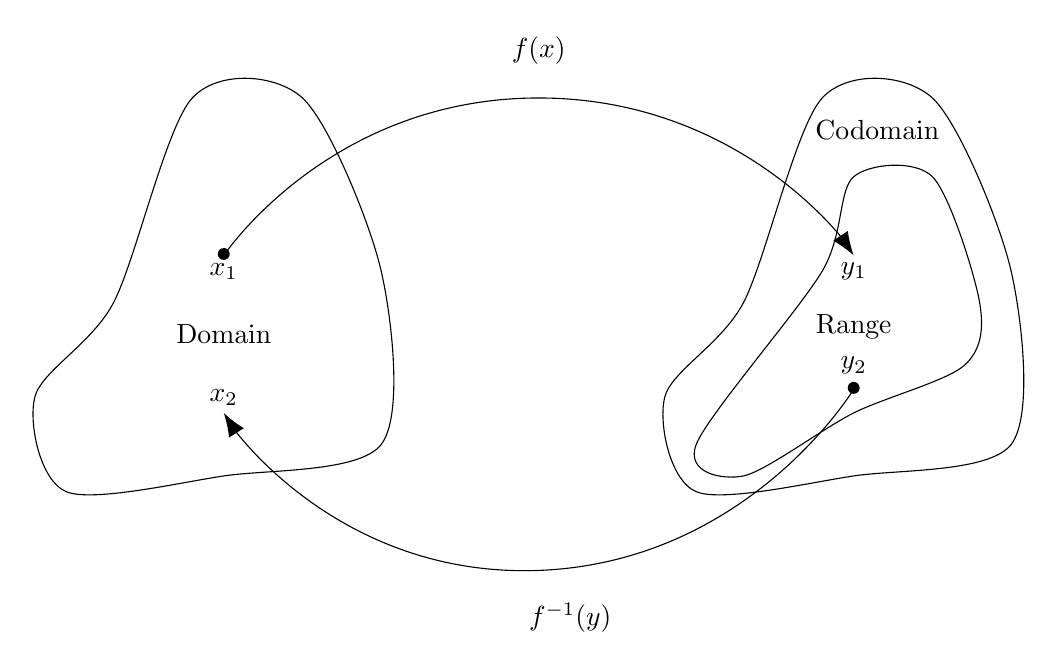
\begin{tikzpicture}[scale=2, filled dot/.style = {anchor=base,fill,circle,inner sep=0.5pt}]
        \draw plot [smooth cycle] coordinates {(0,0) (1,0.1) (2,0.3) (2,1.4) (1.5,2.5) (0.8,2.5) (0.3,1.2) (-0.2,0.6) } node at (1,1) {Domain};
        \draw plot [smooth cycle] coordinates {(4,0) (5,0.1) (6,0.3) (6,1.4) (5.5,2.5) (4.8,2.5) (4.3,1.2) (3.8,0.6) } node at (5.15,2.3) {Codomain};
        \draw plot [smooth cycle] coordinates {(4.3,0.1) (5,0.5) (5.7,0.8) (5.8,1.2) (5.5,2) (5,2) (4.8,1.4) (4,0.3) } node at (5,1.05) {Range};
        \draw[-{Latex[length=3mm]}] plot [smooth,tension=1.2] coordinates {(1,1.5) (3,2.5) (5,1.5)} node at (3,2.8) {$f(x)$} node [filled dot] at (1,1.5){.}  node at (1,1.4) {$x_1$} node at (5,1.4) {$y_1$};
        \draw[-{Latex[length=3mm]}] plot [smooth,tension=1.2] coordinates {(5,0.65) (3,-0.5) (1,0.5)} node at (3.2,-0.8) {$f^{-1}(y)$} node [filled dot] at (5,0.65){.}  node at (5,0.8) {$y_2$} node at (1,0.6) {$x_2$};
    \end{tikzpicture}
\end{center}


\begin{problem}
    What is the difference between the codomain and the range of a function?
    \begin{multipleChoice}
        \choice[correct]{The codomain is the type of thing that the output is, whereas the range is the actual achieveable output.}
        \choice{The range is the type of thing that the output is, whereas the codomain is the actual achieveable output.}
        \choice{The codomain and the range are the same, so there is no difference.}
        \choice{The codomain is the input, and the range is the output of a function.}
        \choice{The codomain is the achieveable output of a function, and the range is the input of the inverse function.}
    \end{multipleChoice}
\end{problem}

By using the range of $f(x)$ as the domain of $f^{-1}(y)$, we make sure that every point in the domain of $f^{-1}(y)$ is defined. Another way to say this is that we only consider the `points that actually came from some $x$-value' when we reverse the relationship to make the inverse relation.
    
    
    Here is a video with more!
    
    \youtube{tgEUPCJ-SKk}
    

\end{document}